\documentclass[
	fontsize=12pt,
	paper=a4,
	twoside=false,
	numbers=noenddot,
	plainheadsepline,
	toc=listof,
	toc=bibliography
]{scrartcl}

\usepackage[english]{babel} 

\usepackage[round]{natbib}

\usepackage{amssymb,amsmath}

\usepackage{placeins}
\usepackage{float}

\usepackage{graphicx}
\restylefloat{figure}
\usepackage{subfigure} 

\usepackage{array}

\usepackage{hyperref}

\setlength{\parindent}{0pt}

\title{Result of testing RANSAC approach for wheel detection}


\begin{document}

\maketitle


To test the RANSAC approach for wheel detection we selected for each possible configuration of settings (mouse ID, time of recording and network ID) one video from the given data set. The results of total $28$ Videos are presented below.

% ------------------------------------------------------------------------------------------
\section*{Mouse $1$}
% ------------------------------------------------------------------------------------------

%\subsection*{ $1$ day p.o.}

\begin{figure} [htb]
	\centering
	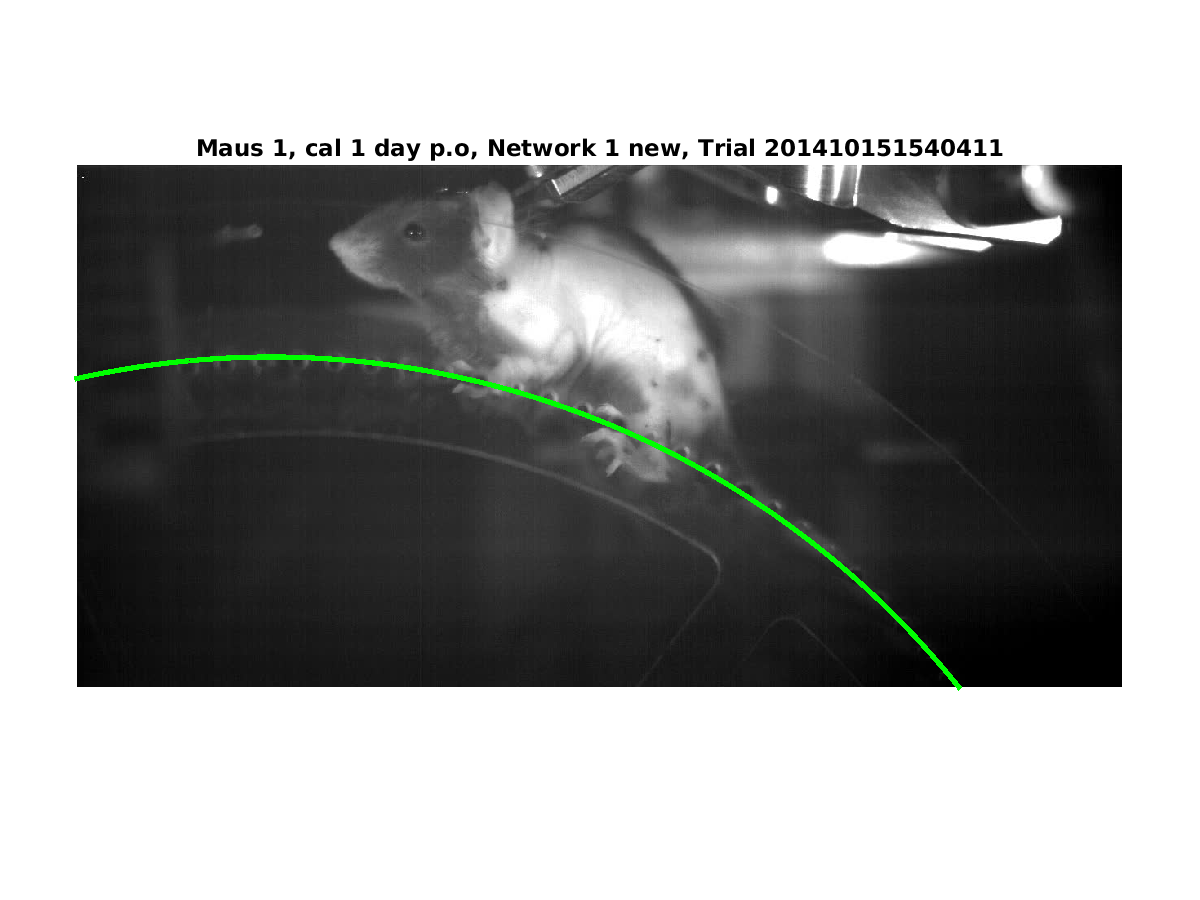
\includegraphics[scale = 0.6]{images/mouse1/result_Maus_1_cal_1_day_Network_1_new.png}
\end{figure}
\begin{figure} [htb] \centering
	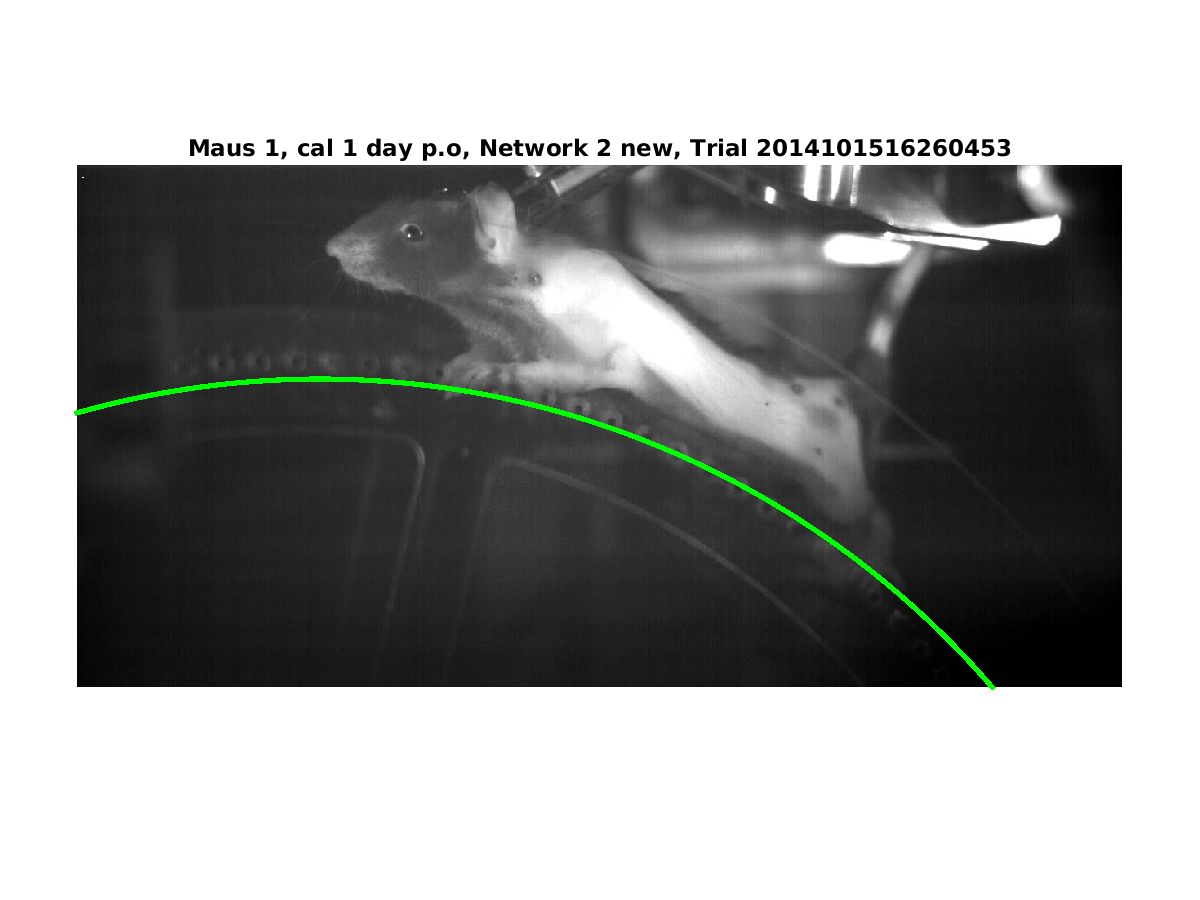
\includegraphics[scale = 0.6]{images/mouse1/result_Maus_1_cal_1_day_Network_2_new.png}
\end{figure}

%\FloatBarrier

%\subsection*{ $5$ day p.o.}

\begin{figure} [hb] \centering
	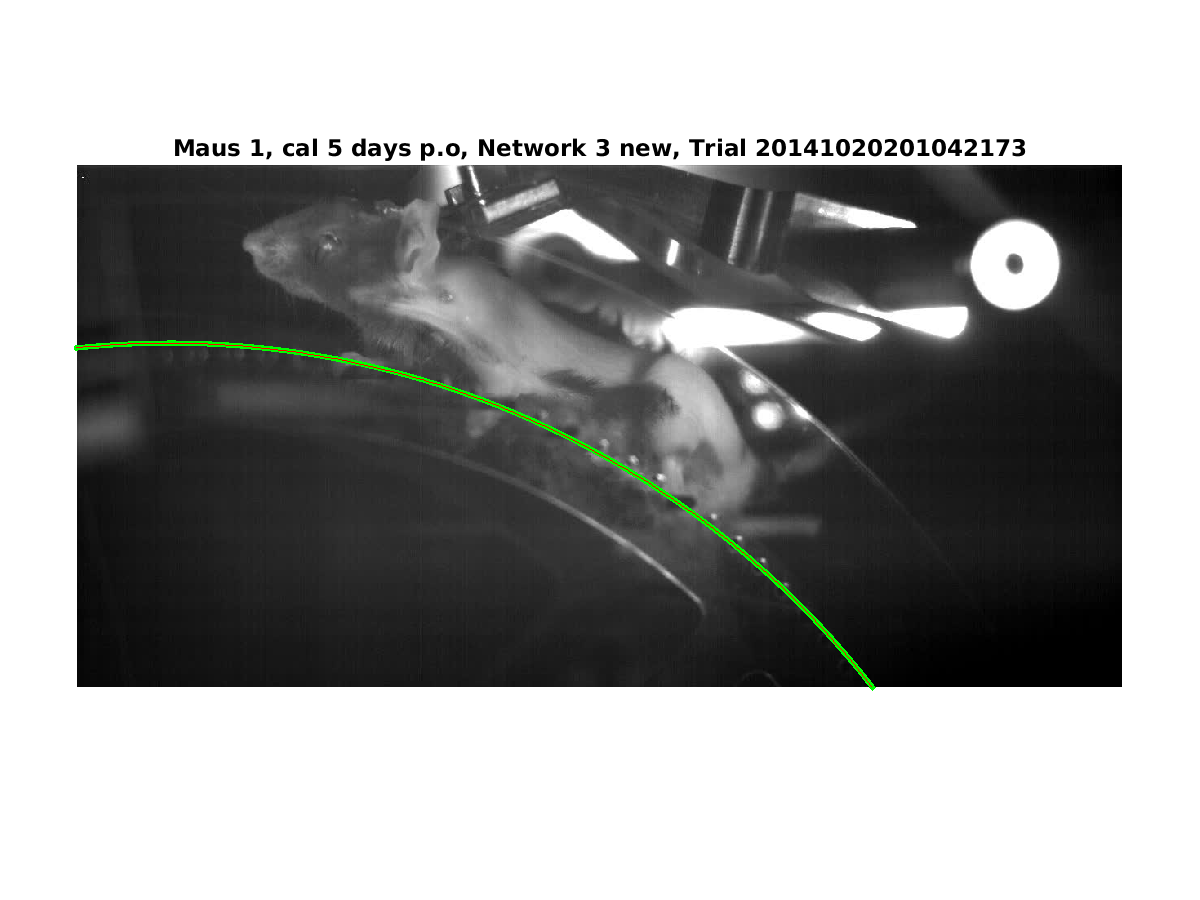
\includegraphics[scale = 0.6]{images/mouse1/result_Maus_1_cal_5_days_Network_3_new_2.png}
\end{figure}
\begin{figure} [htb] \centering
	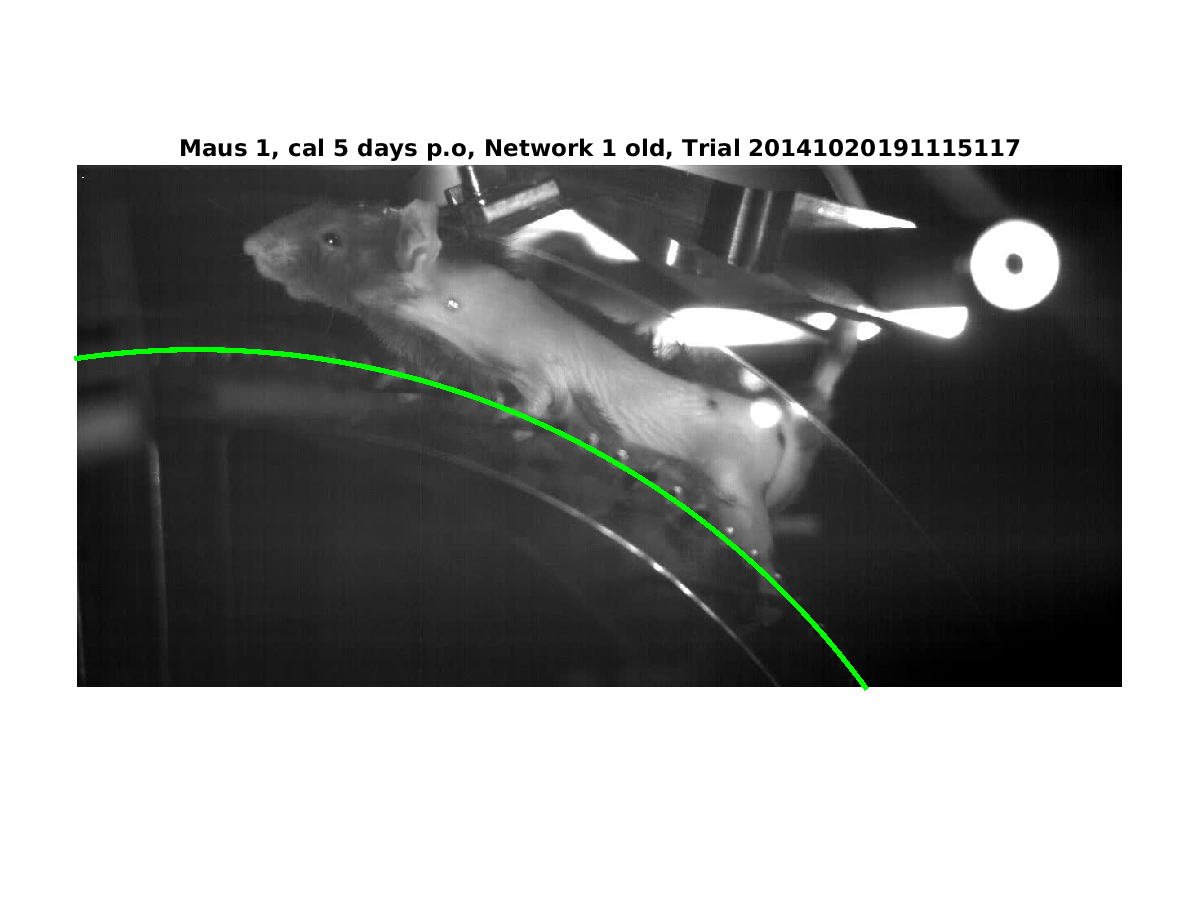
\includegraphics[scale = 0.6]{images/mouse1/result_Maus_1_cal_5_days_Network_1_old.png}
\end{figure}

%\FloatBarrier

%\subsection*{ $4$ weeks p.o.}

\begin{figure} [htb] \centering
	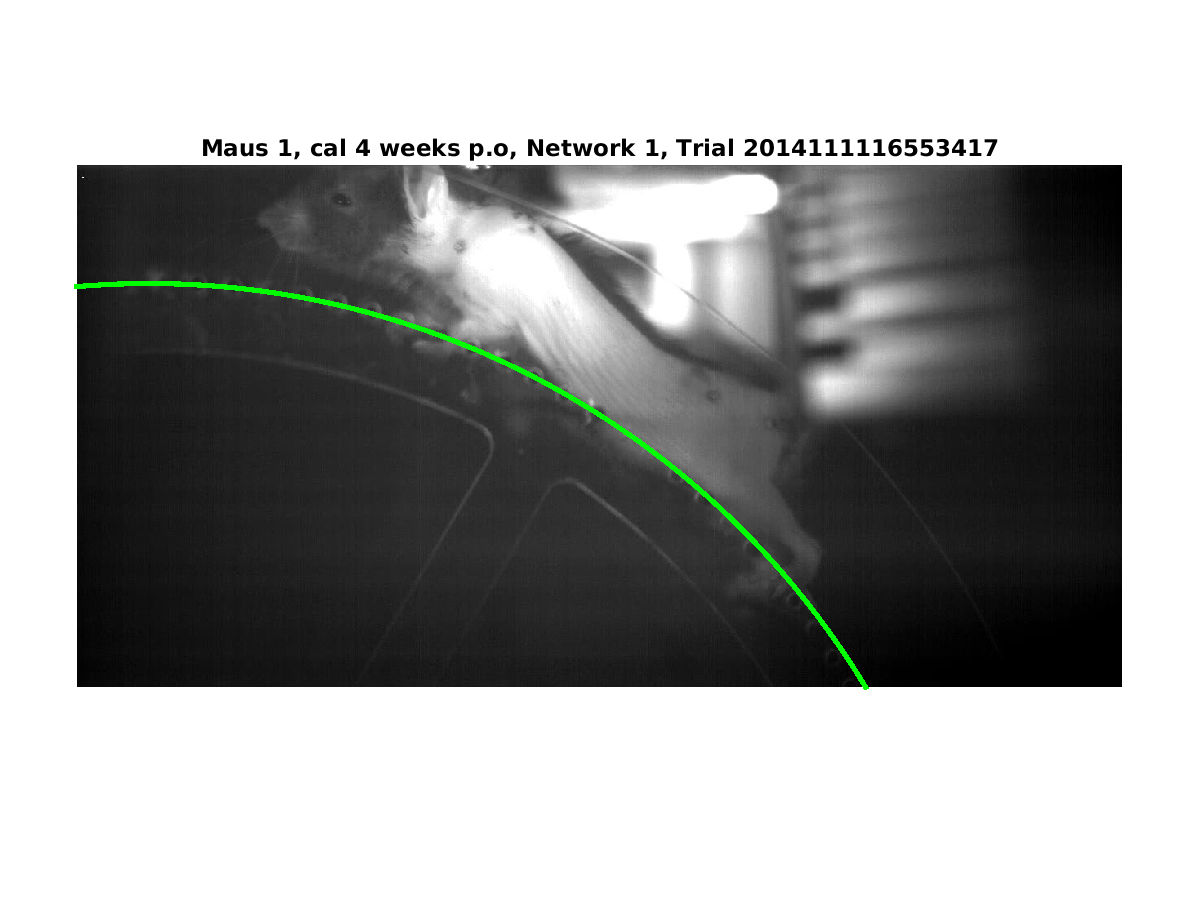
\includegraphics[scale = 0.6]{images/mouse1/result_Maus_1_cal_4_weeks_Network_1.png}
\end{figure}
\begin{figure} [htb] \centering
	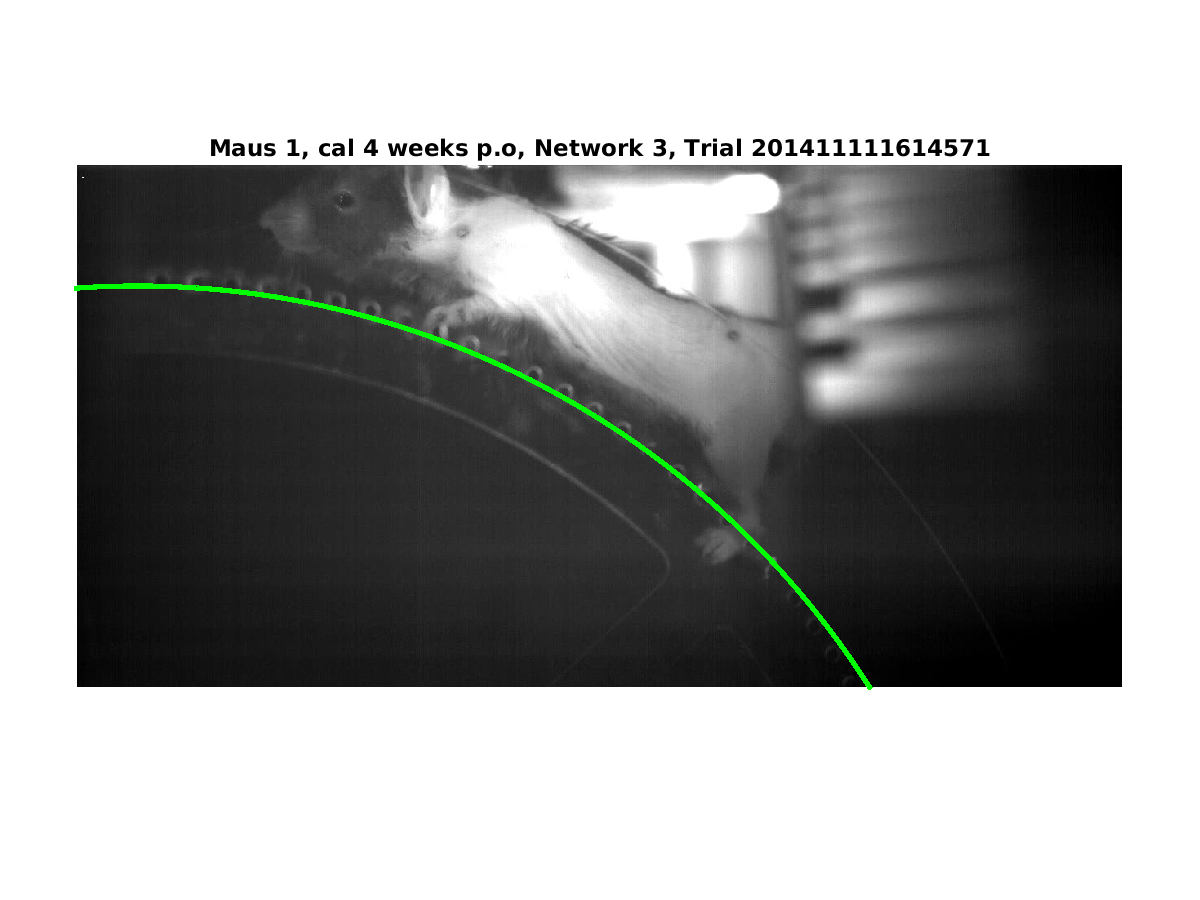
\includegraphics[scale = 0.6]{images/mouse1/result_Maus_1_cal_4_weeks_Network_3.png}
\end{figure}
\begin{figure} [htb] \centering
	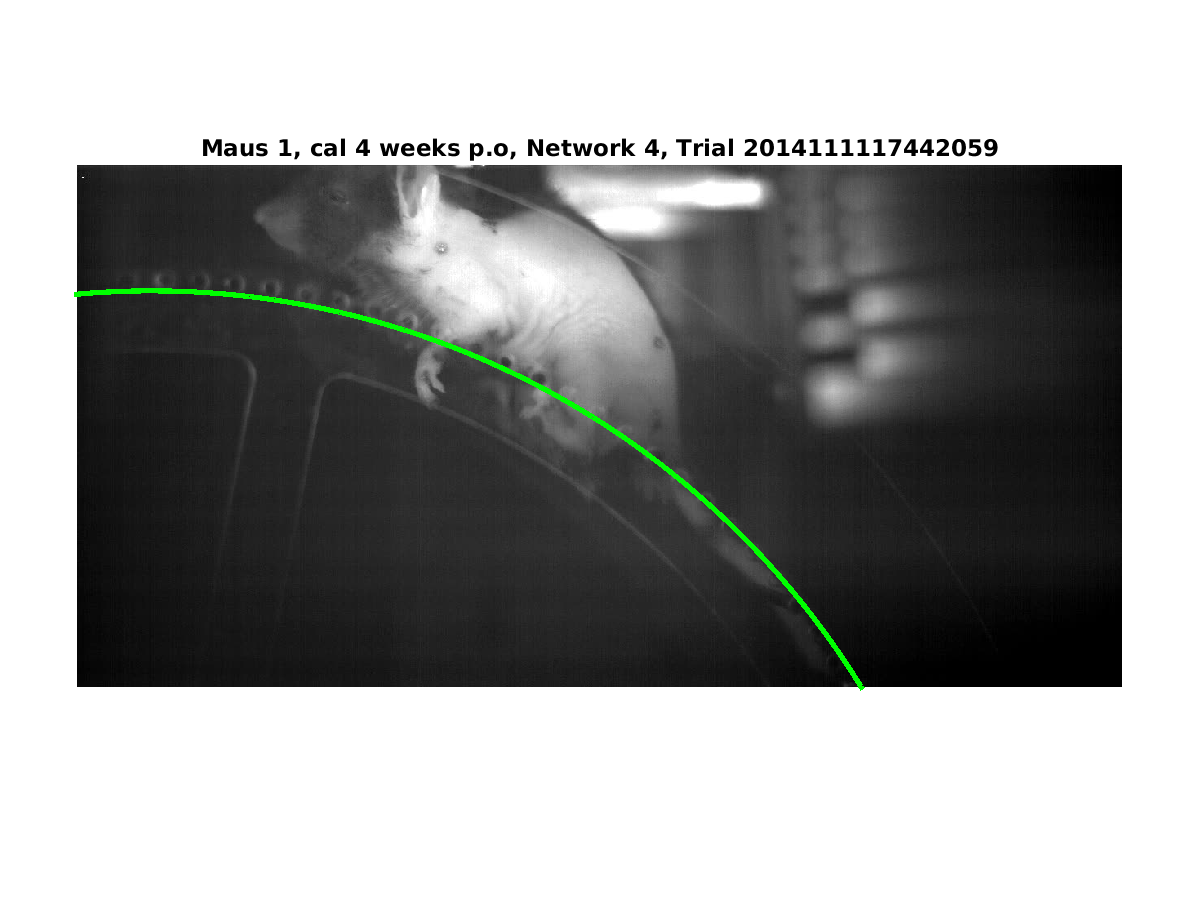
\includegraphics[scale = 0.6]{images/mouse1/result_Maus_1_cal_4_weeks_Network_4.png}
\end{figure}

\FloatBarrier

% ------------------------------------------------------------------------------------------
\section*{Mouse $2$}
% ------------------------------------------------------------------------------------------
%\subsection*{ $1$ day p.o.}

\begin{figure} [htb]
	\centering
	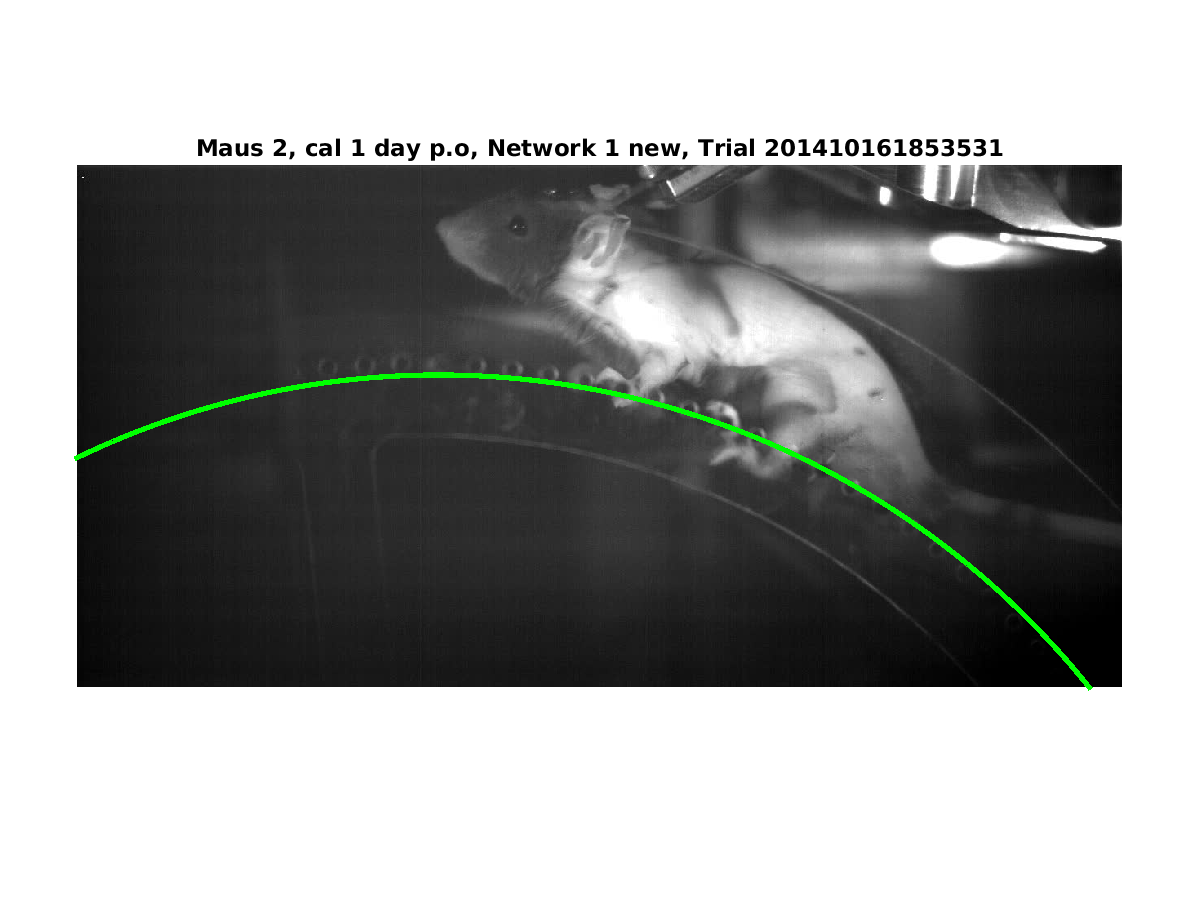
\includegraphics[scale = 0.6]{images/mouse2/result_Maus_2_cal_1_day_Network_1_new.png}
\end{figure}
\begin{figure} [hb] \centering
	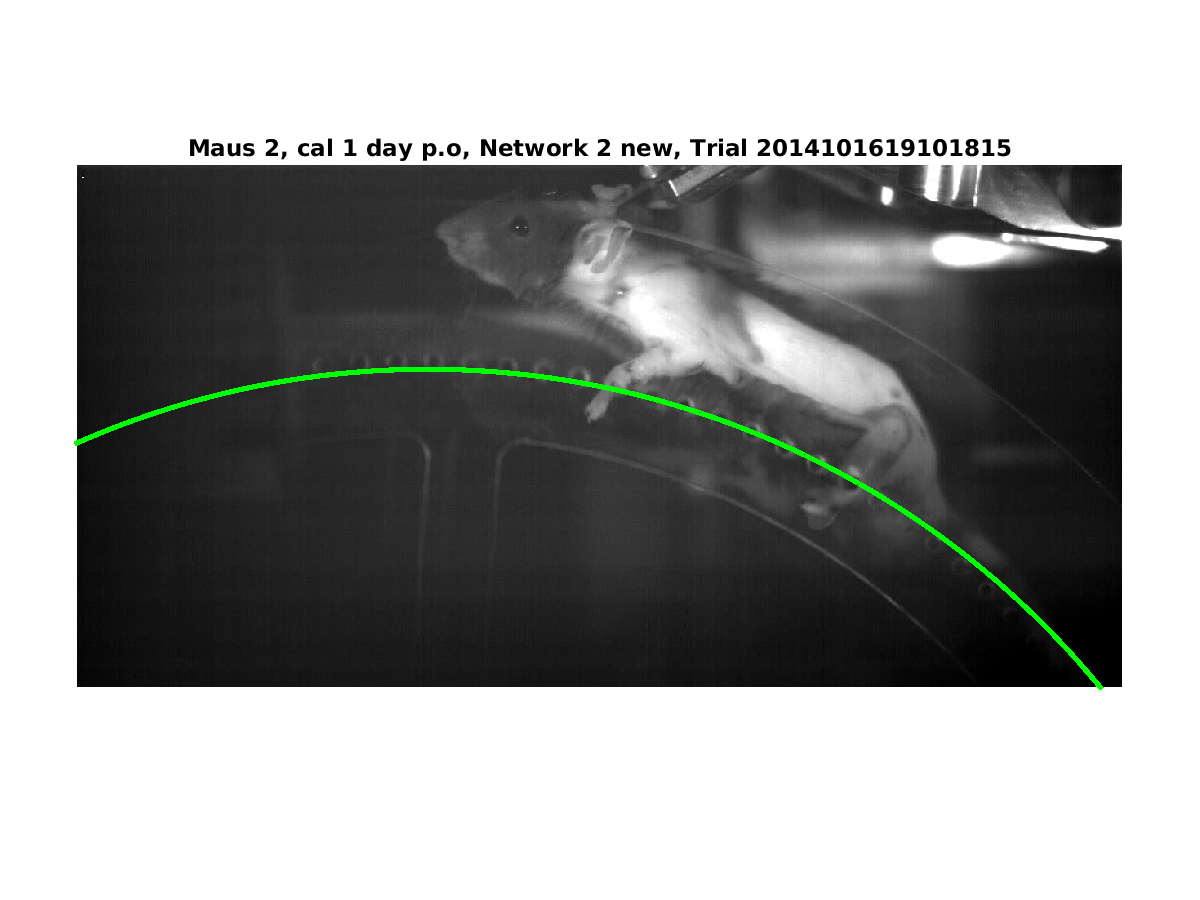
\includegraphics[scale = 0.6]{images/mouse2/result_Maus_2_cal_1_day_Network_2_new.png}
\end{figure}

%\FloatBarrier

%\subsection*{ $5$ day p.o.}

\begin{figure} [hb] \centering
	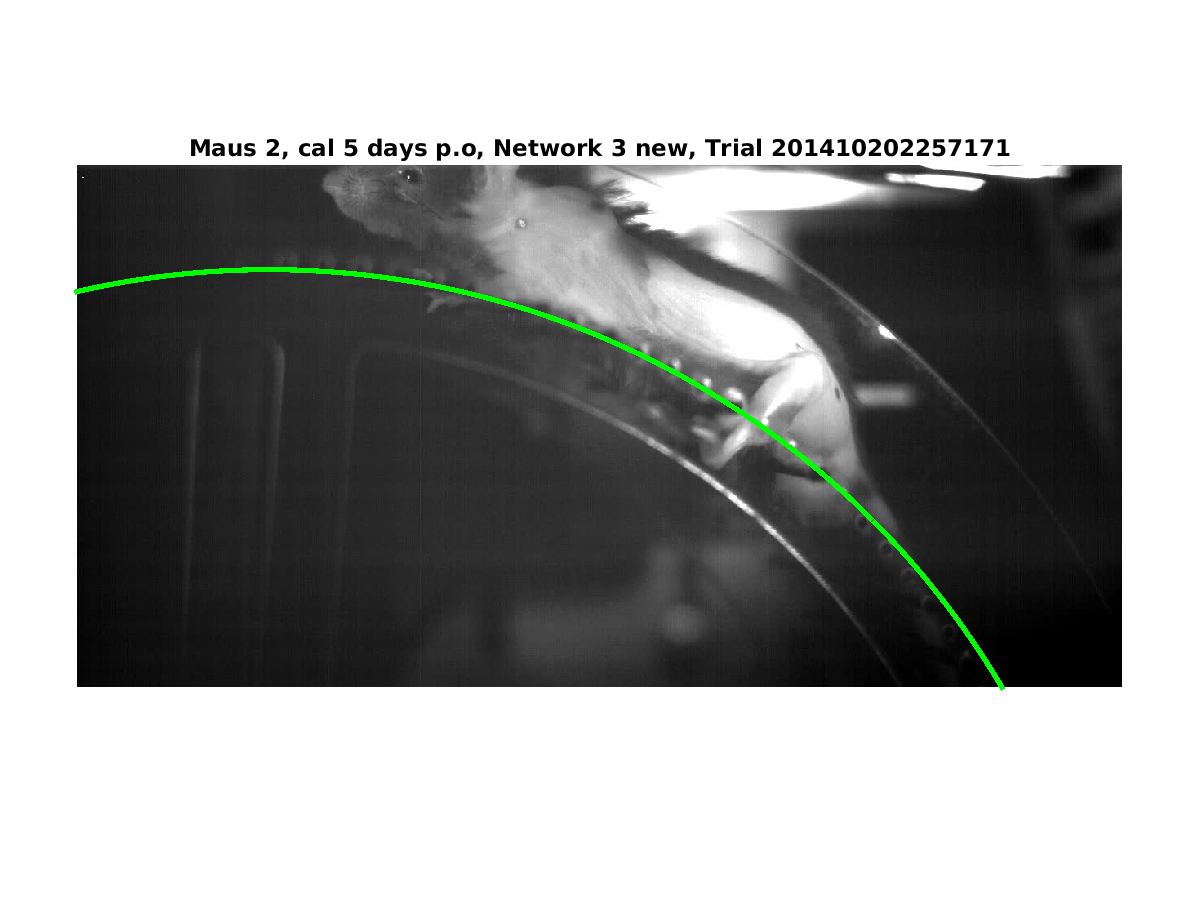
\includegraphics[scale = 0.6]{images/mouse2/result_Maus_2_cal_5_days_Network_3_new.png}
\end{figure}
\begin{figure} [htb] \centering
	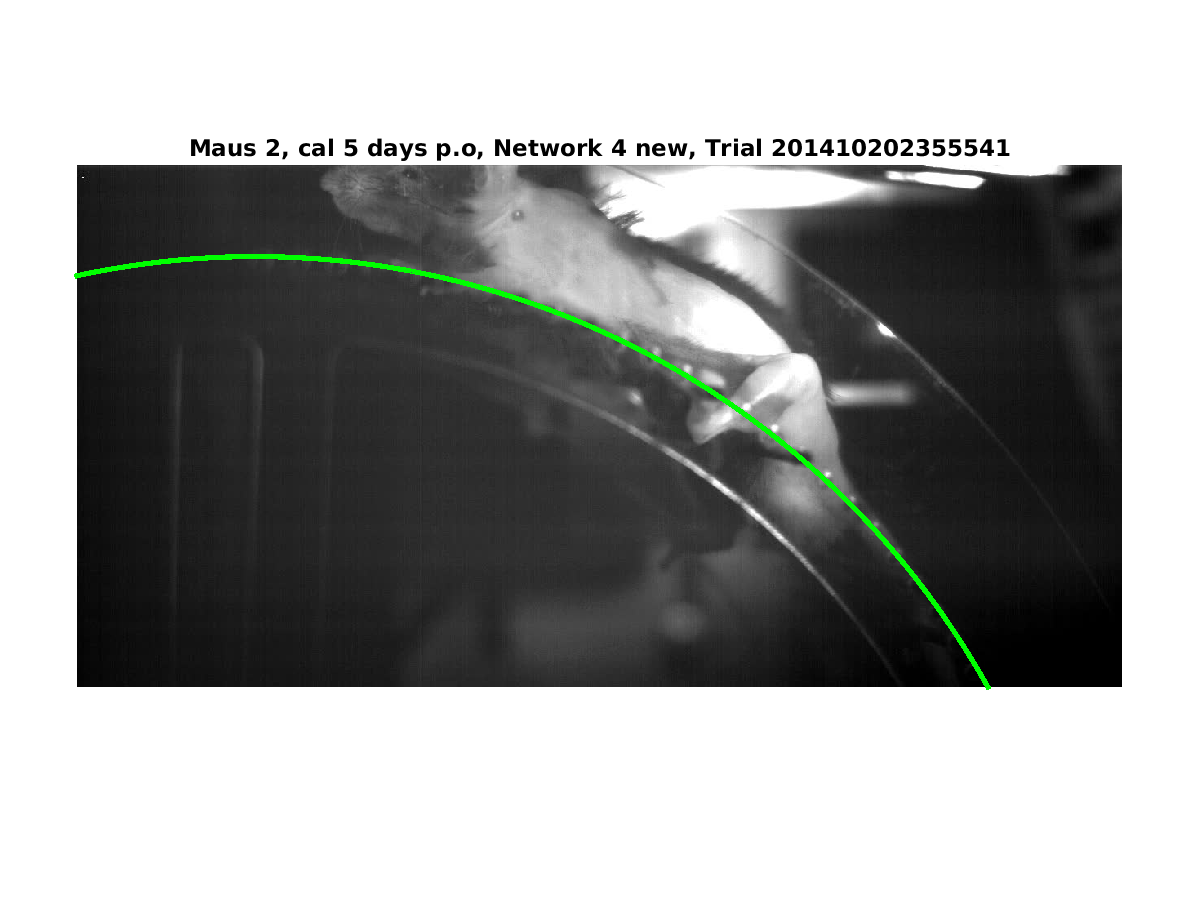
\includegraphics[scale = 0.6]{images/mouse2/result_Maus_2_cal_5_days_Network_4_new.png}
\end{figure}

%\FloatBarrier

%\subsection*{ $4$ weeks p.o.}

\FloatBarrier



% ------------------------------------------------------------------------------------------
\section*{Mouse $3$}
% ------------------------------------------------------------------------------------------

%\subsection*{ $1$ day p.o.}

\begin{figure} [htb]
	\centering
	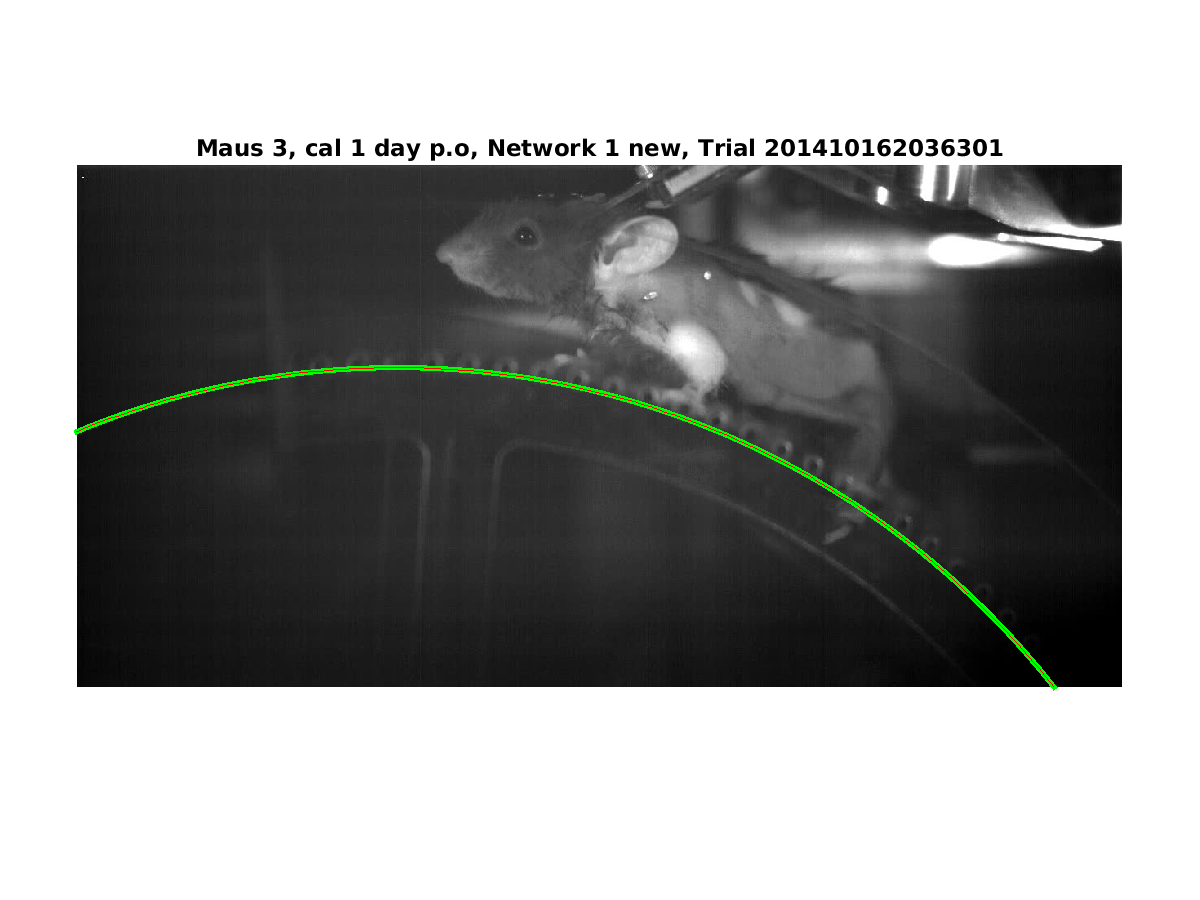
\includegraphics[scale = 0.6]{images/mouse3/result_Maus_3_cal_1_day_Network_1_new_2.png}
\end{figure}
\begin{figure} [htb] \centering
	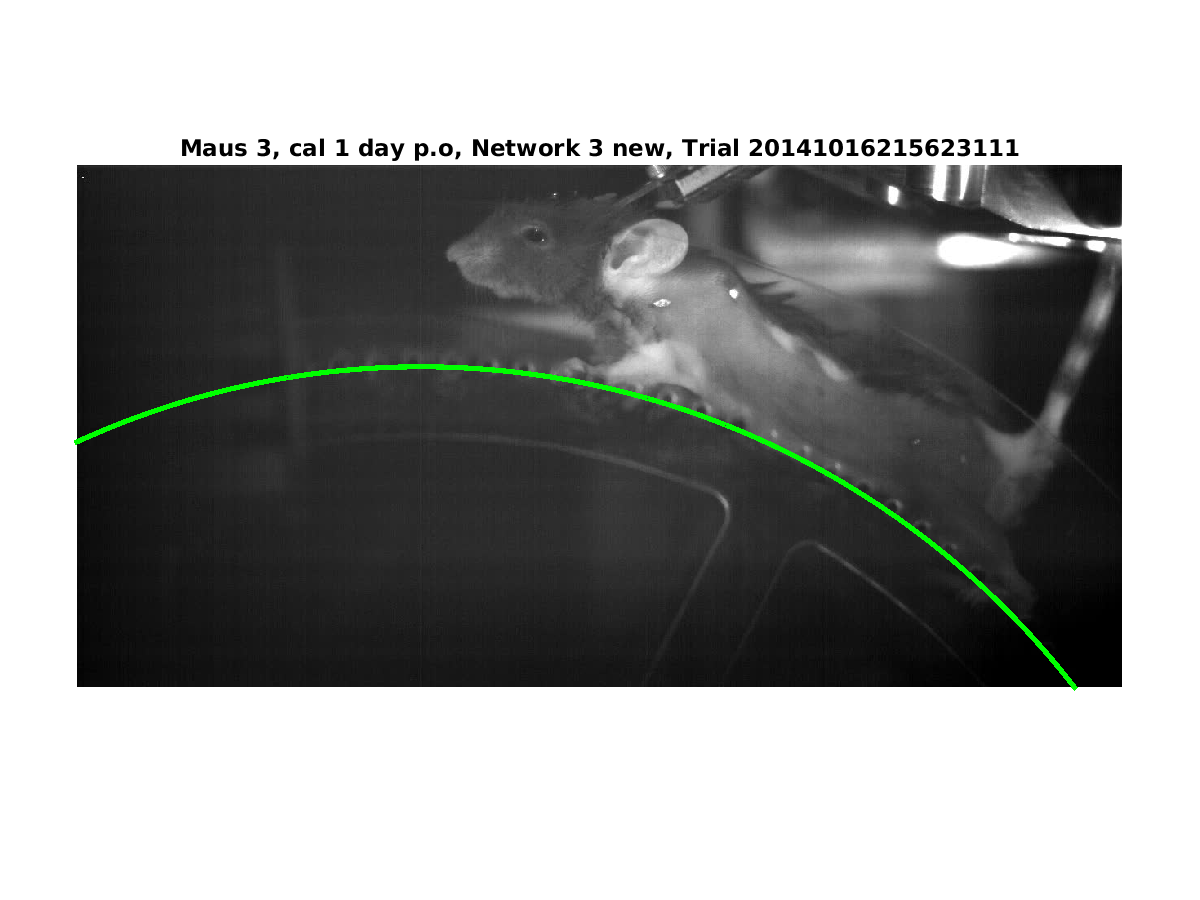
\includegraphics[scale = 0.6]{images/mouse3/result_Maus_3_cal_1_day_Network_3_new.png}
\end{figure}

%\FloatBarrier

%\subsection*{ $5$ day p.o.}

\begin{figure} [htb] \centering
	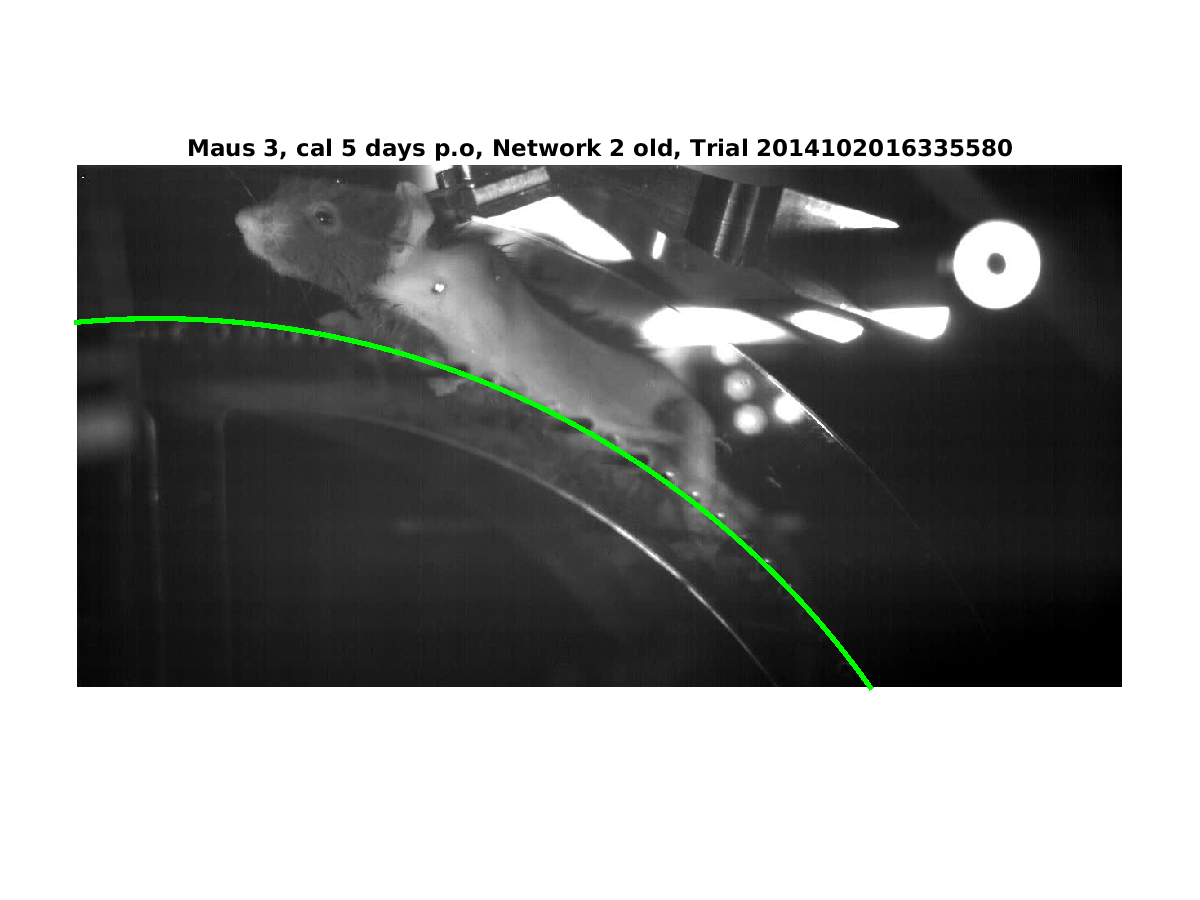
\includegraphics[scale = 0.6]{images/mouse3/result_Maus_3_cal_5_days_Network_2_old.png}
\end{figure}

%\FloatBarrier

%\subsection*{ $4$ weeks p.o.}

\begin{figure} [htb] \centering
	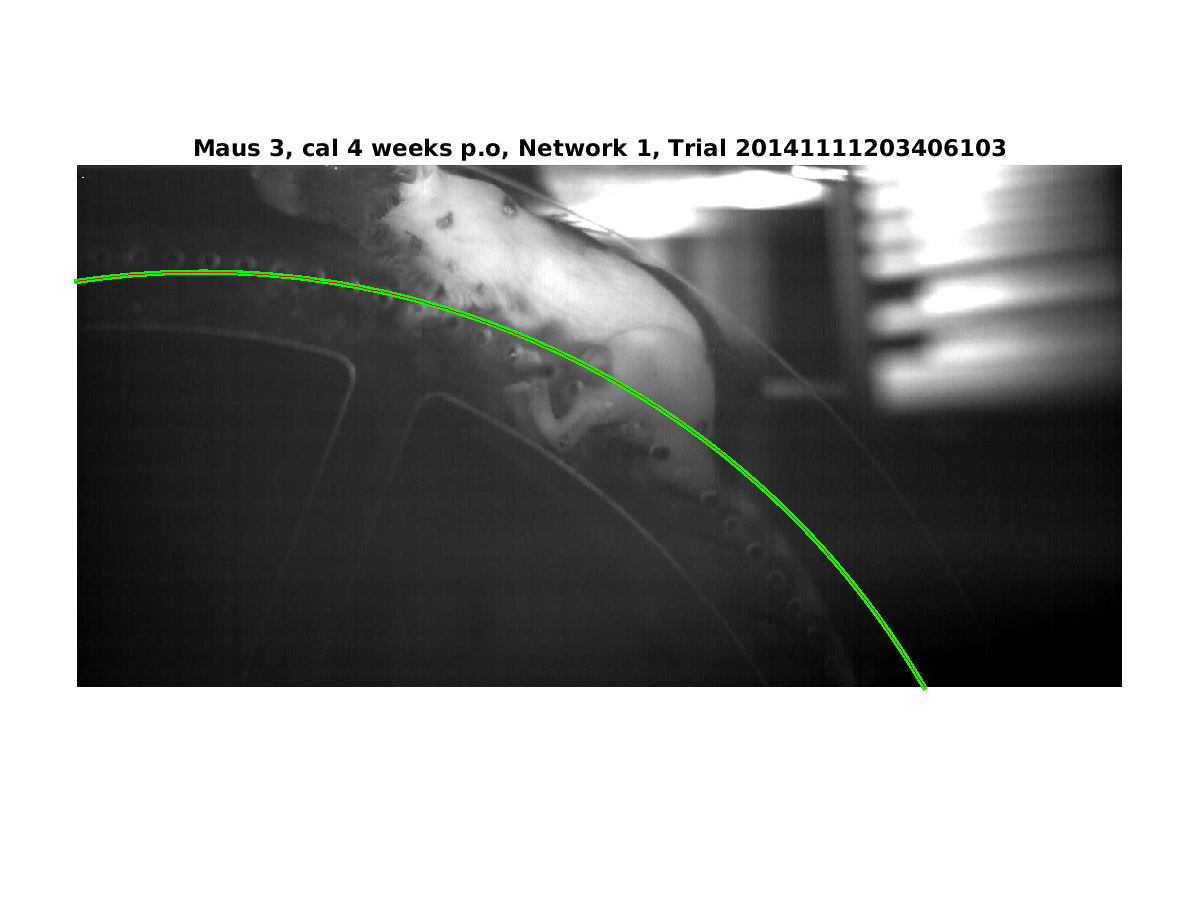
\includegraphics[scale = 0.6]{images/mouse3/result_Maus_3_cal_4_weeks_Network_1_2.png}
\end{figure}
\begin{figure} [htb] \centering
	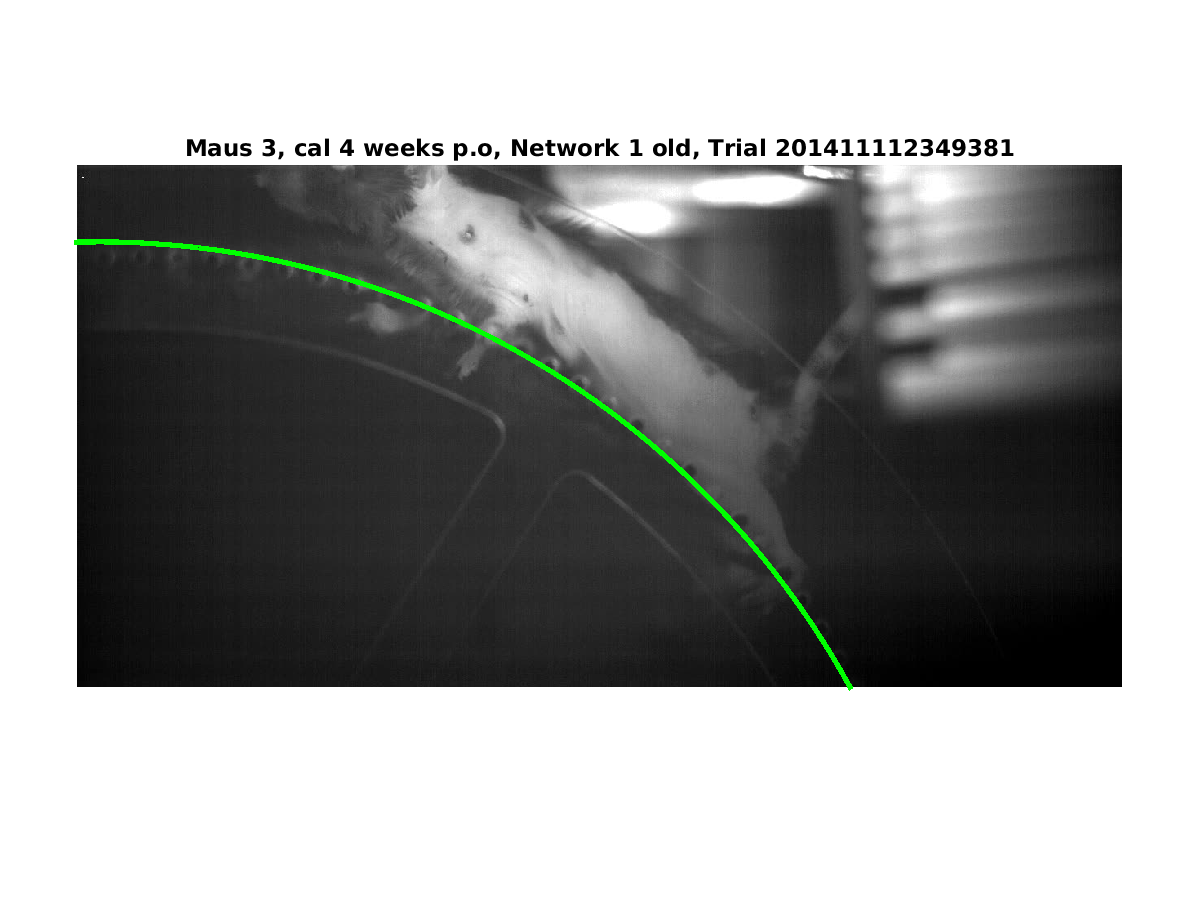
\includegraphics[scale = 0.6]{images/mouse3/result_Maus_3_cal_4_weeks_Network_1_old.png}
\end{figure}
\begin{figure} [htb] \centering
	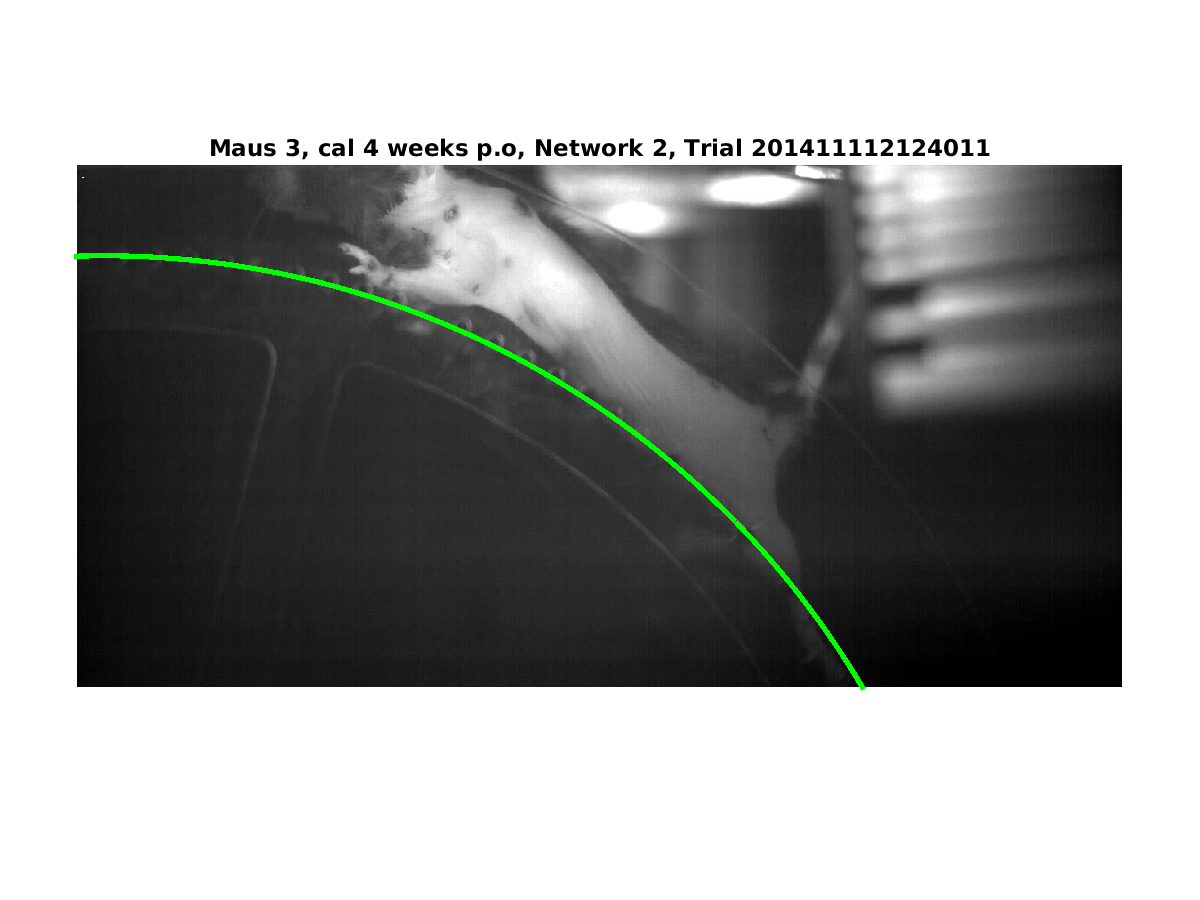
\includegraphics[scale = 0.6]{images/mouse3/result_Maus_3_cal_4_weeks_Network_2.png}
\end{figure}
\begin{figure} [htb] \centering
	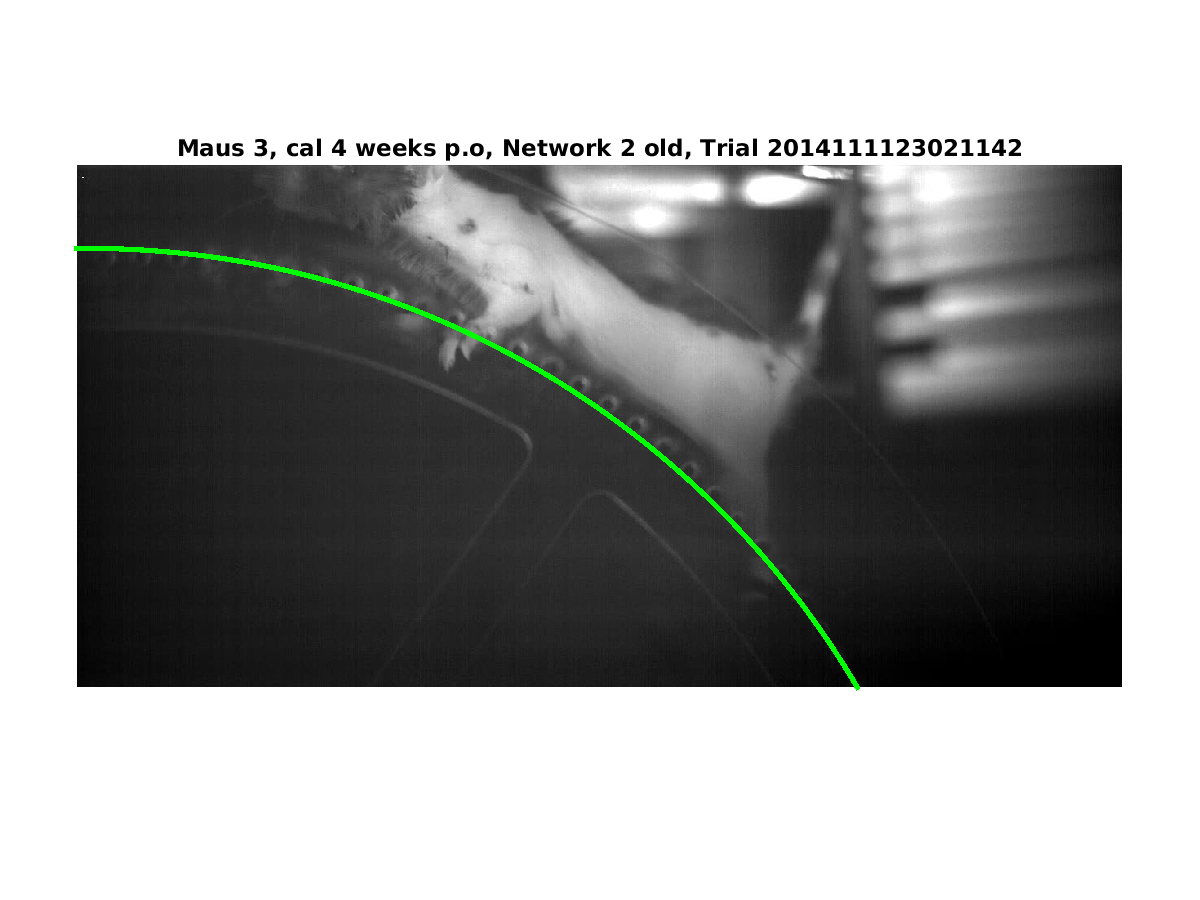
\includegraphics[scale = 0.6]{images/mouse3/result_Maus_3_cal_4_weeks_Network_2_old.png}
\end{figure}

\FloatBarrier

% ------------------------------------------------------------------------------------------
\section*{Mouse $4$}
% ------------------------------------------------------------------------------------------

%\subsection*{ $1$ day p.o.}

\begin{figure} [htb]
	\centering
	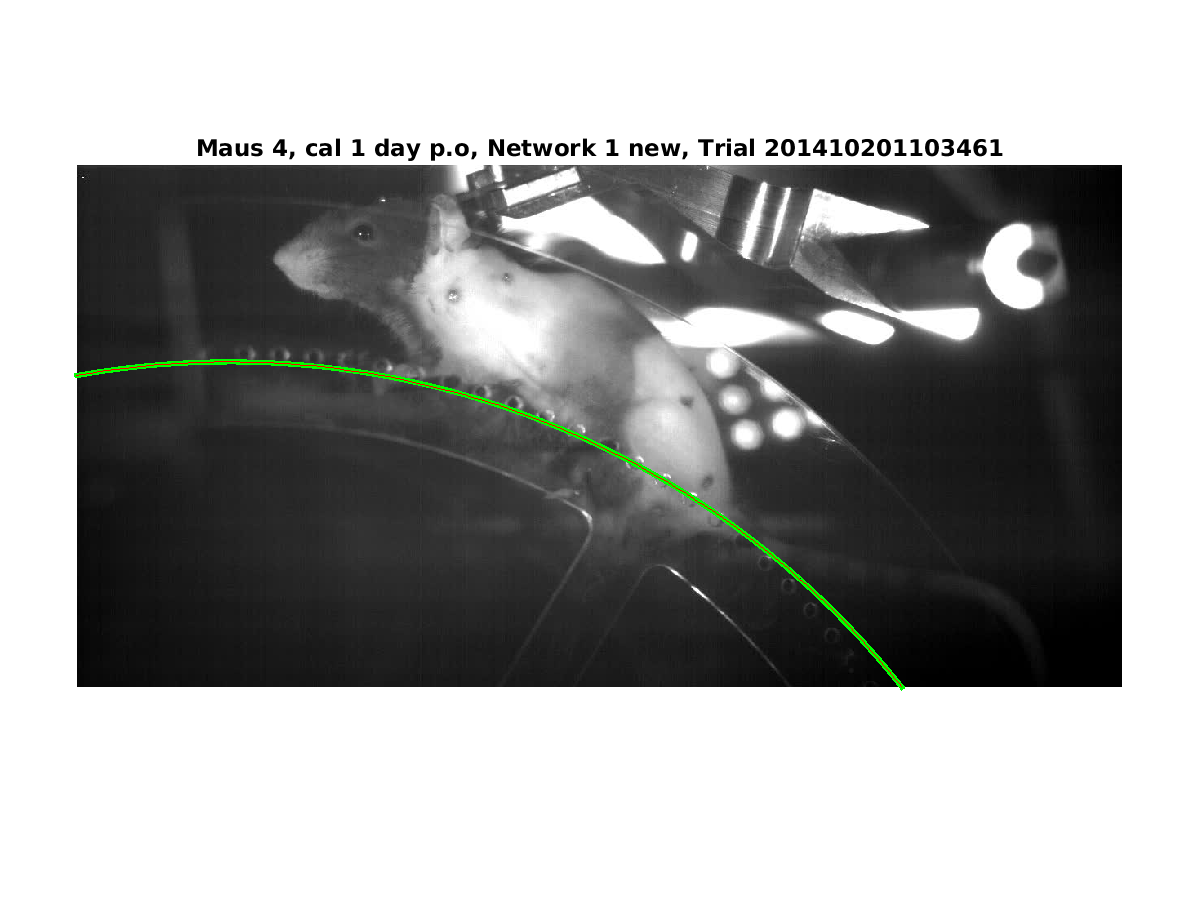
\includegraphics[scale = 0.6]{images/mouse4/result_Maus_4_cal_1_day_Network_1_new_2.png}
\end{figure}
\begin{figure} [htb] \centering
	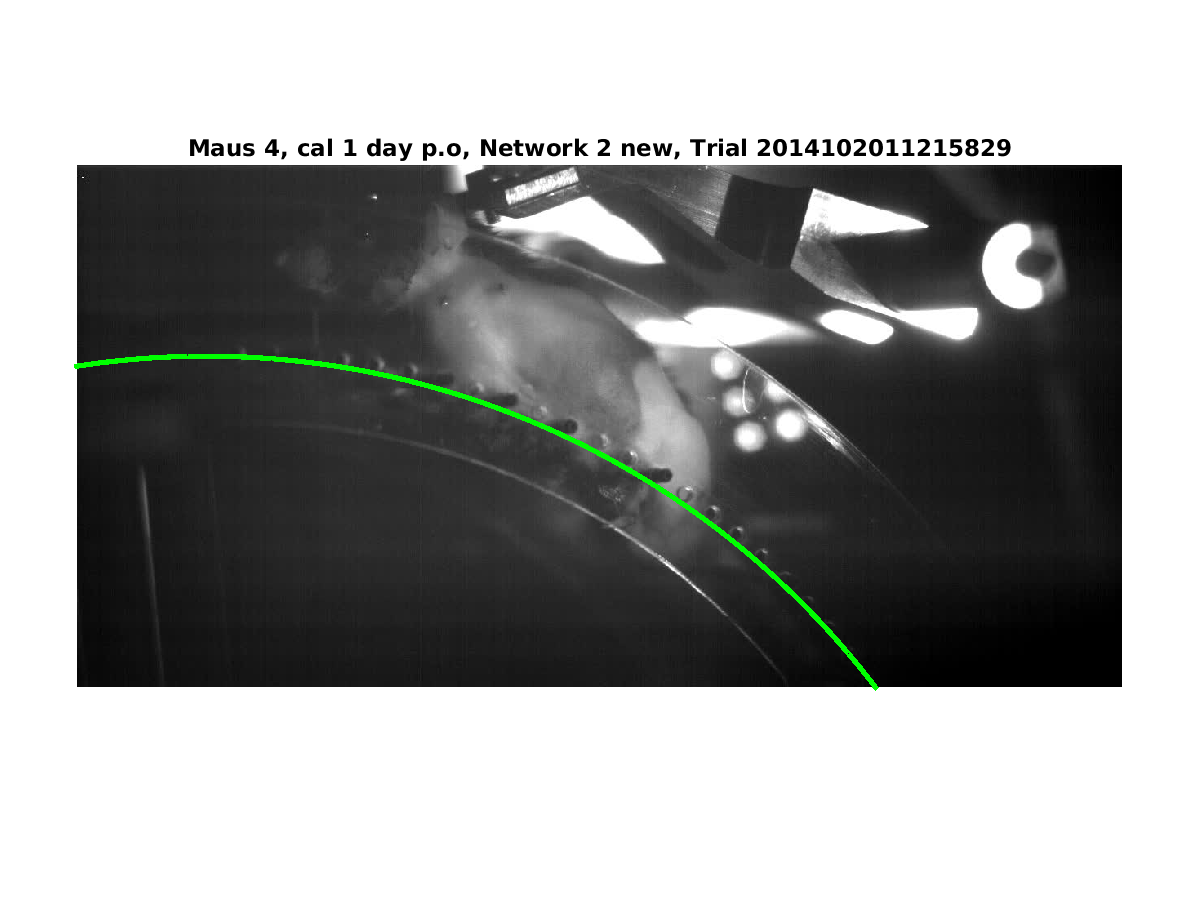
\includegraphics[scale = 0.6]{images/mouse4/result_Maus_4_cal_1_day_Network_2_new.png}
\end{figure}
\begin{figure} [htb] \centering
	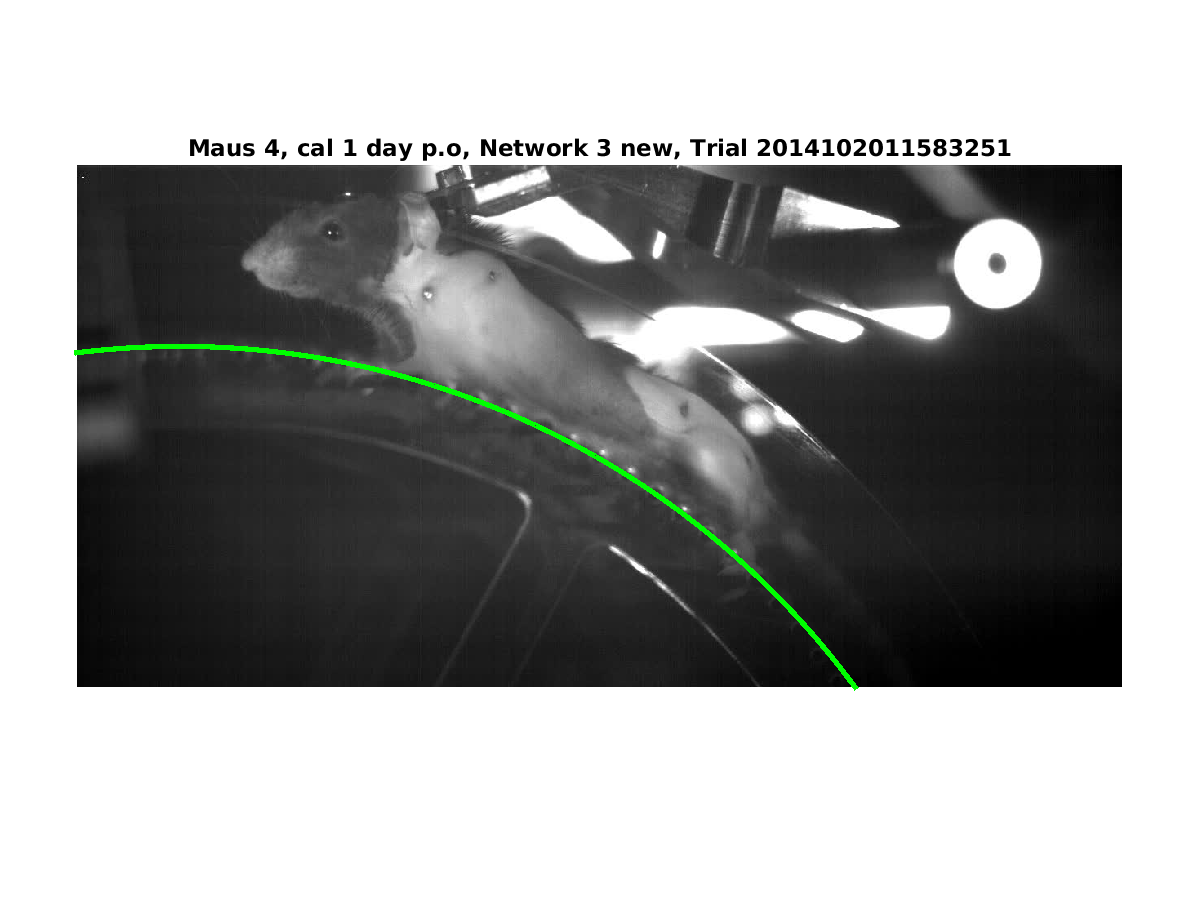
\includegraphics[scale = 0.6]{images/mouse4/result_Maus_4_cal_1_day_Network_3_new.png}
\end{figure}
\begin{figure} [htb] \centering
	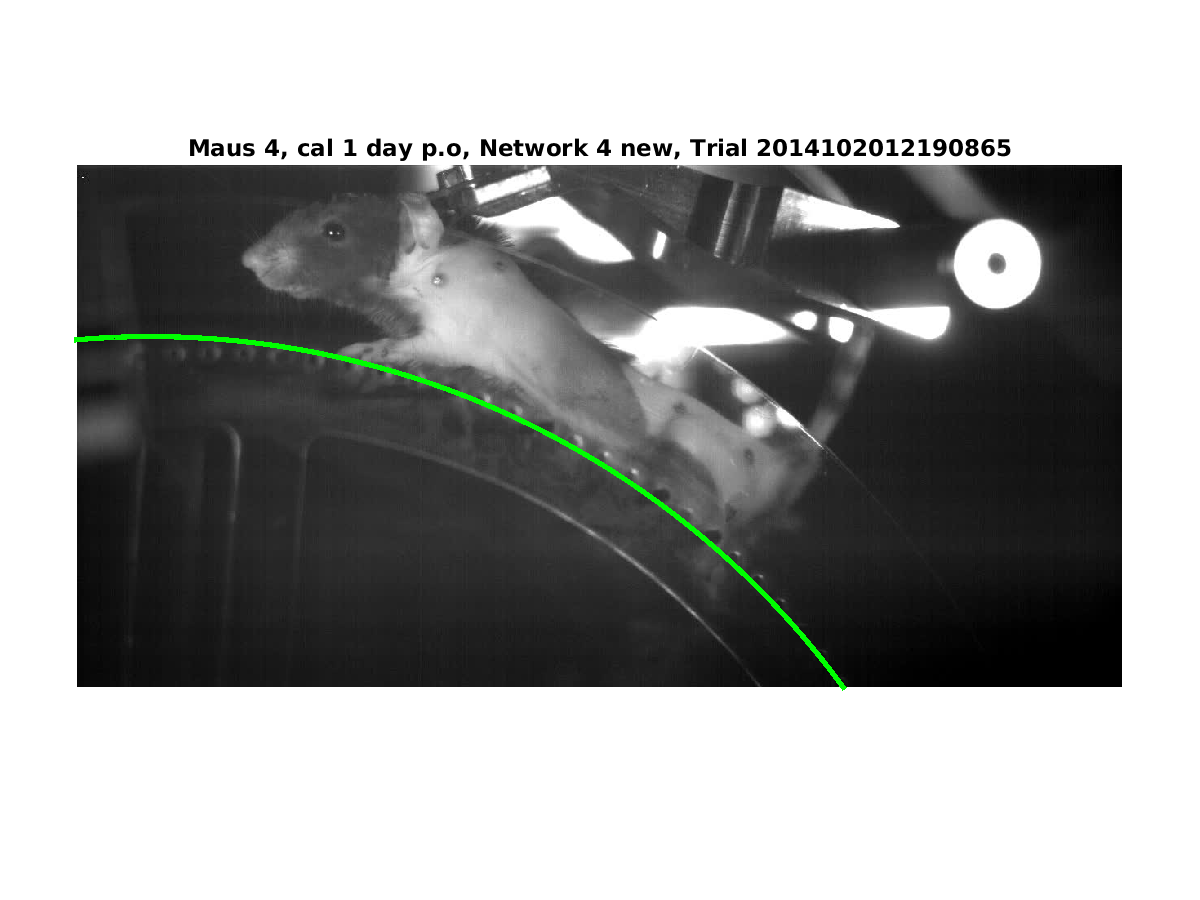
\includegraphics[scale = 0.6]{images/mouse4/result_Maus_4_cal_1_day_Network_4_new.png}
\end{figure}


%\FloatBarrier

%\subsection*{ $5$ day p.o.}


%\FloatBarrier

%\subsection*{ $4$ weeks p.o.}

\begin{figure} [htb] \centering
	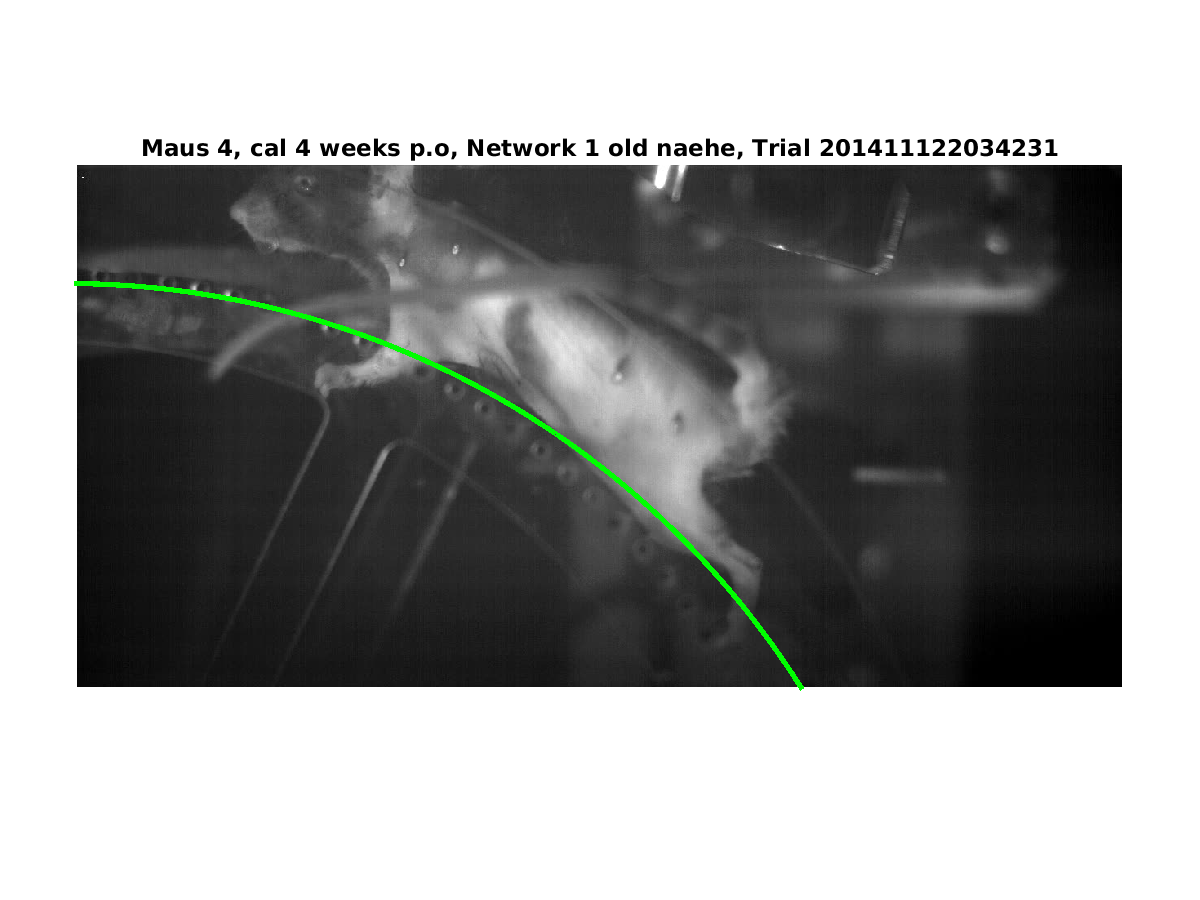
\includegraphics[scale = 0.6]{images/mouse4/result_Maus_4_cal_4_weeks_Network_1_old_naehe.png}
\end{figure}
\begin{figure} [htb] \centering
	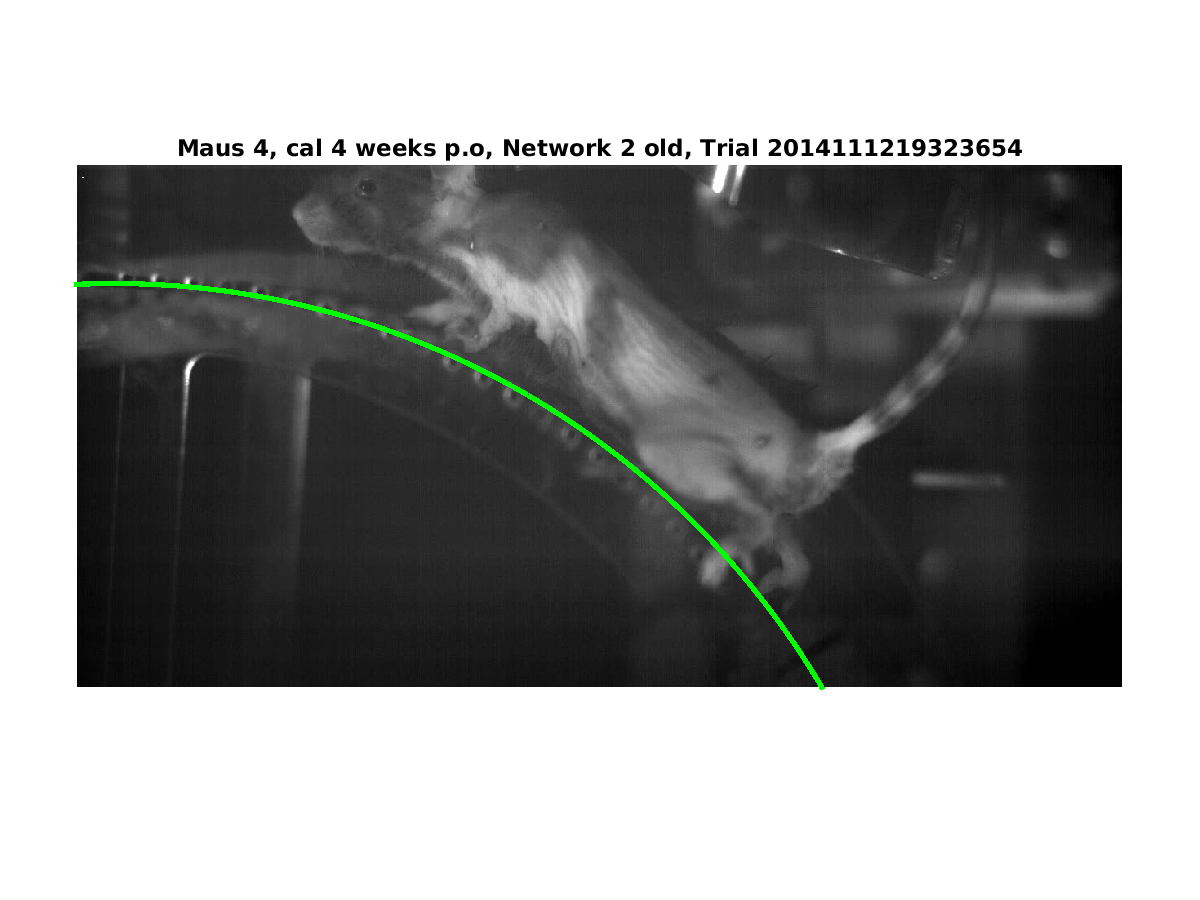
\includegraphics[scale = 0.6]{images/mouse4/result_Maus_4_cal_4_weeks_Network_2_old.png}
\end{figure}
\begin{figure} [htb] \centering
	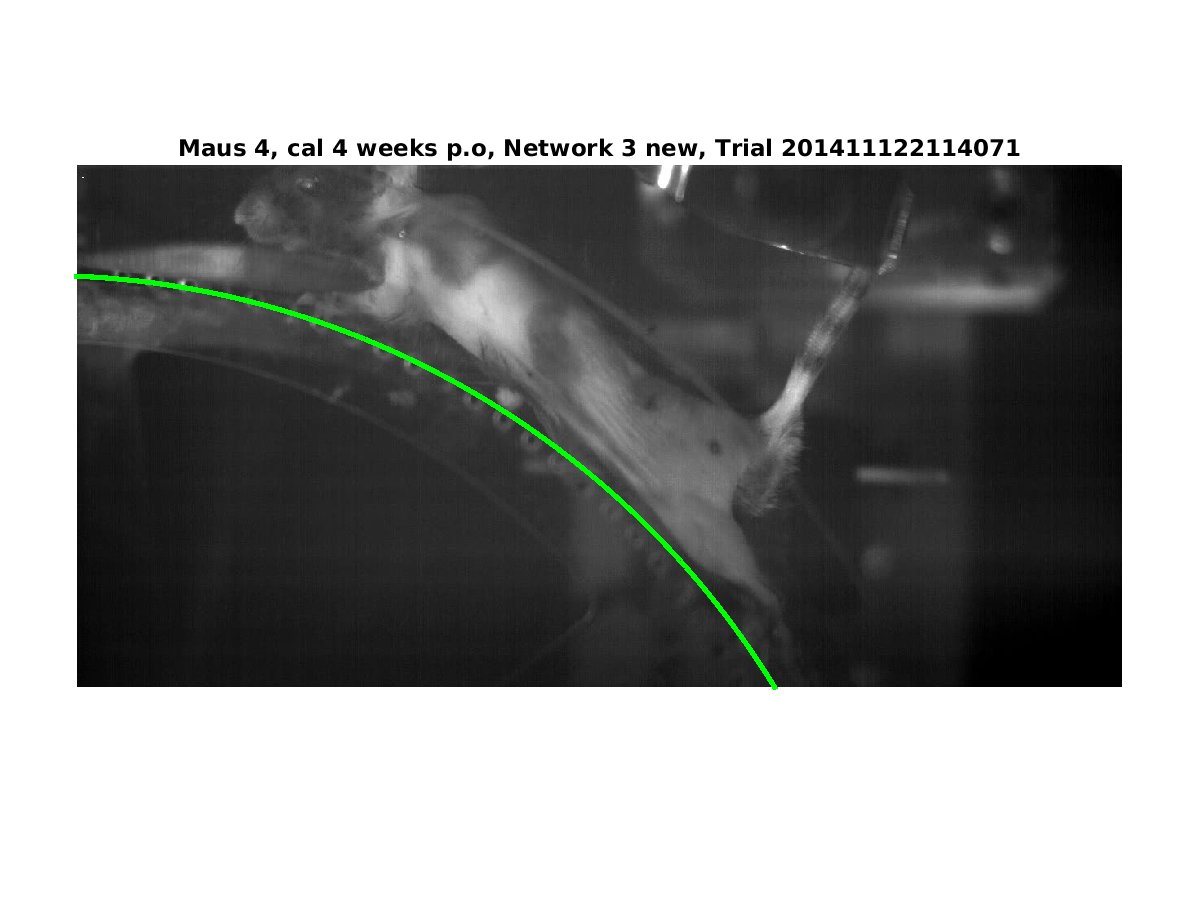
\includegraphics[scale = 0.6]{images/mouse4/result_Maus_4_cal_4_weeks_Network_3_new.png}
\end{figure}

\FloatBarrier

% ------------------------------------------------------------------------------------------
\section*{Mouse $5$}
% ------------------------------------------------------------------------------------------


%\subsection*{ $1$ day p.o.}


%\FloatBarrier

%\subsection*{ $5$ day p.o.}


%\FloatBarrier

%\subsection*{ $4$ weeks p.o.}

\begin{figure} [htb] \centering
	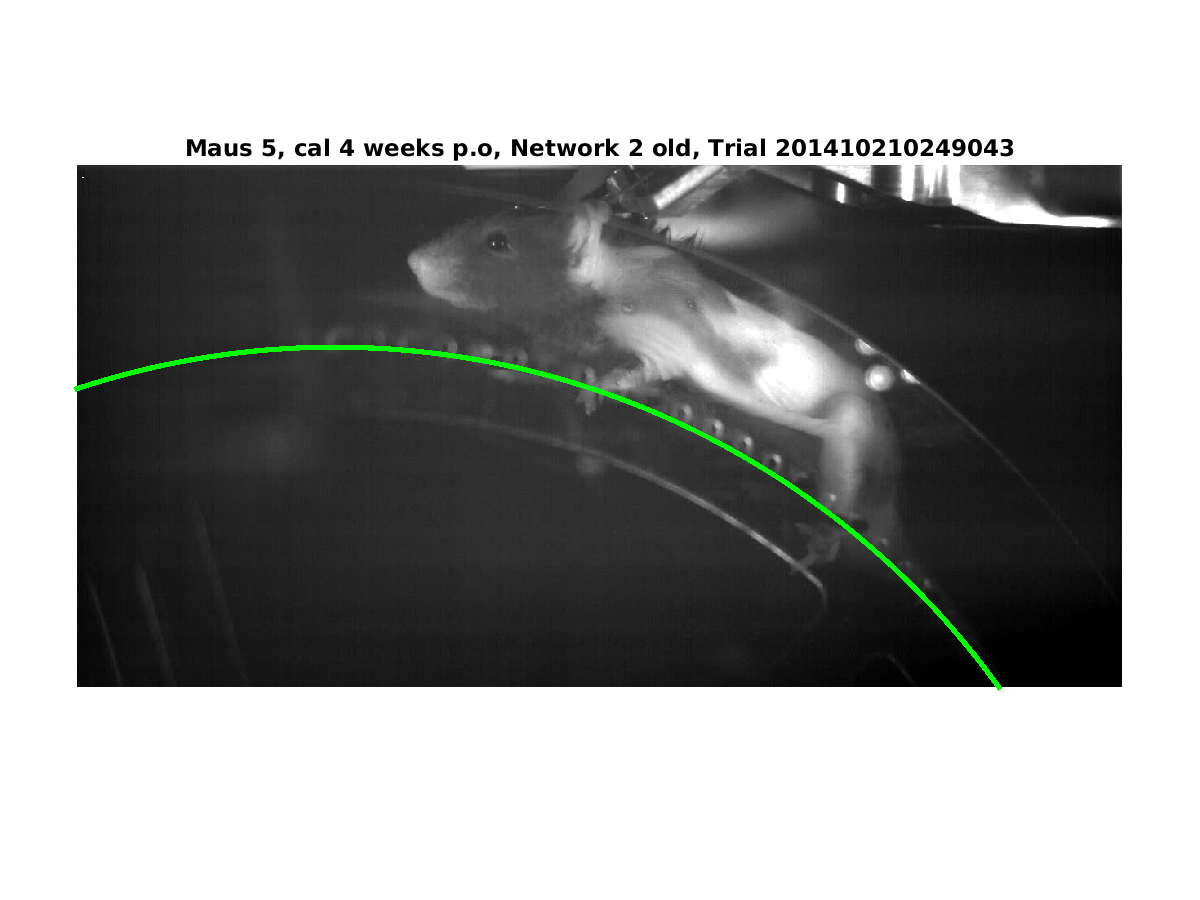
\includegraphics[scale = 0.6]{images/mouse5/result_Maus_5_cal_4_weeks_Network_2_old.png}
\end{figure}
\begin{figure} [htb] \centering
	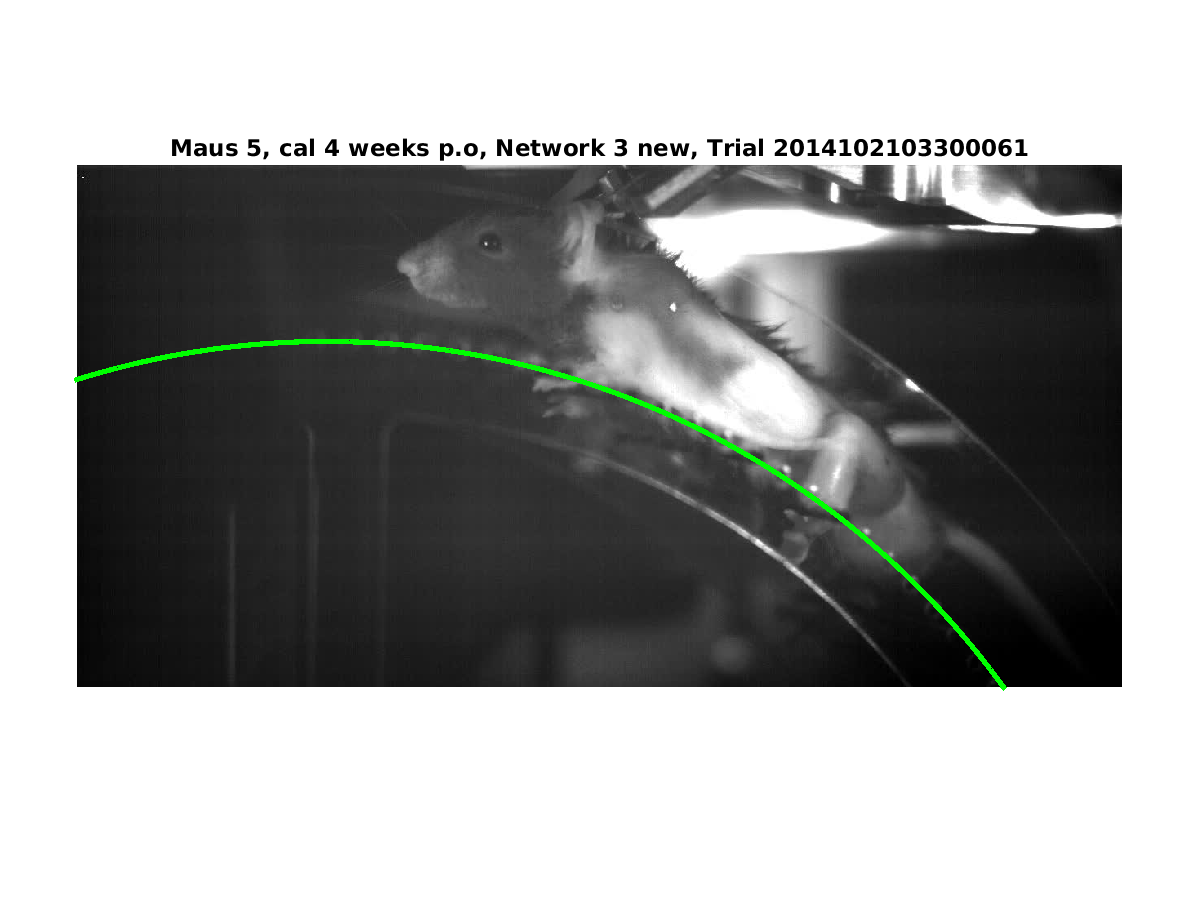
\includegraphics[scale = 0.6]{images/mouse5/result_Maus_5_cal_4_weeks_Network_3_new.png}
\end{figure}
\begin{figure} [htb] \centering
	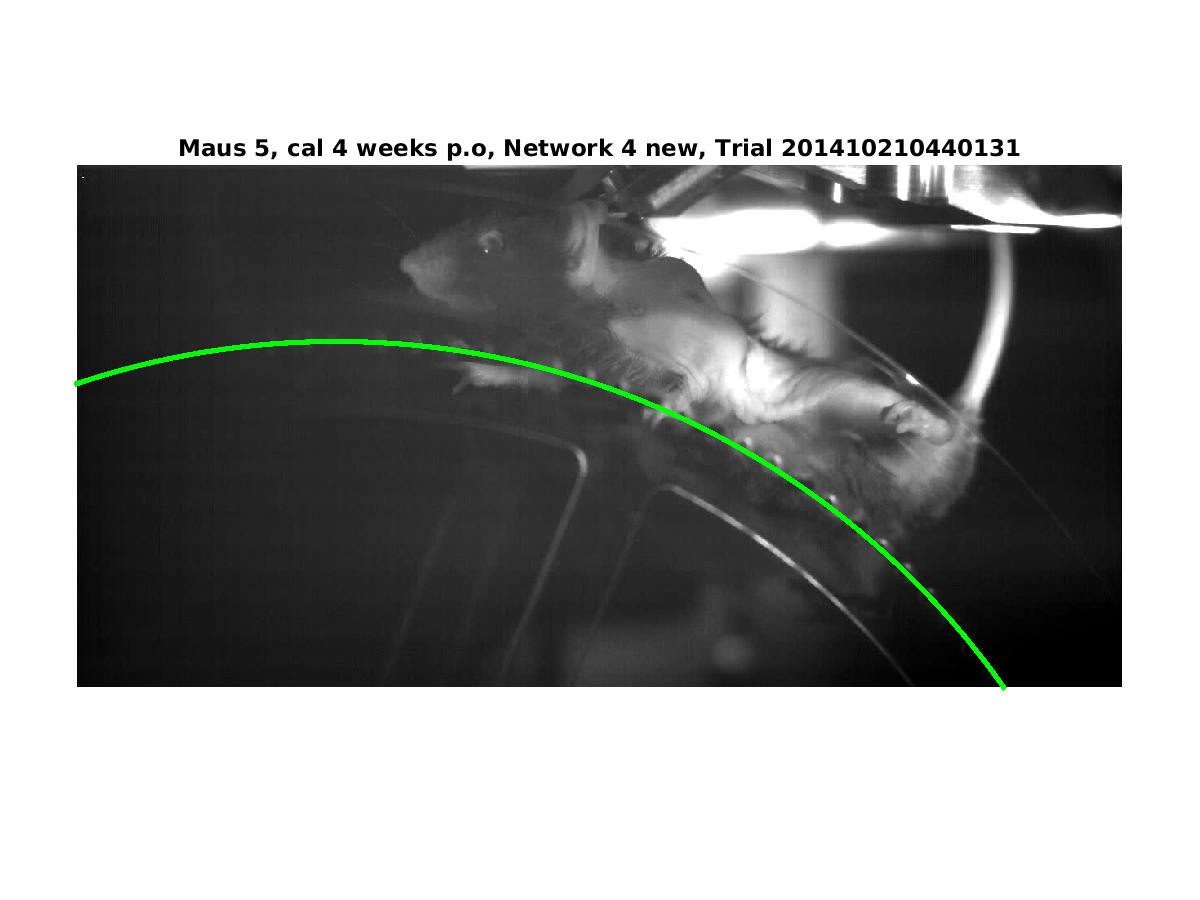
\includegraphics[scale = 0.6]{images/mouse5/result_Maus_5_cal_4_weeks_Network_4_new.png}
\end{figure}

\FloatBarrier

\end{document}